%     #
%    # #   #       ####   ####  #####  # ##### #    # #    #
%   #   #  #      #    # #    # #    # #   #   #    # ##  ##
%  #     # #      #      #    # #    # #   #   ###### # ## #
%  ####### #      #  ### #    # #####  #   #   #    # #    #
%  #     # #      #    # #    # #   #  #   #   #    # #    #
%  #     # ######  ####   ####  #    # #   #   #    # #    #
%
%

%TODO: add legend for domset, etc colors in figure.
%TODO: smaller (a), (b), (c), (d)
% FIGURE 1
\begin{figure*}
 \centering
 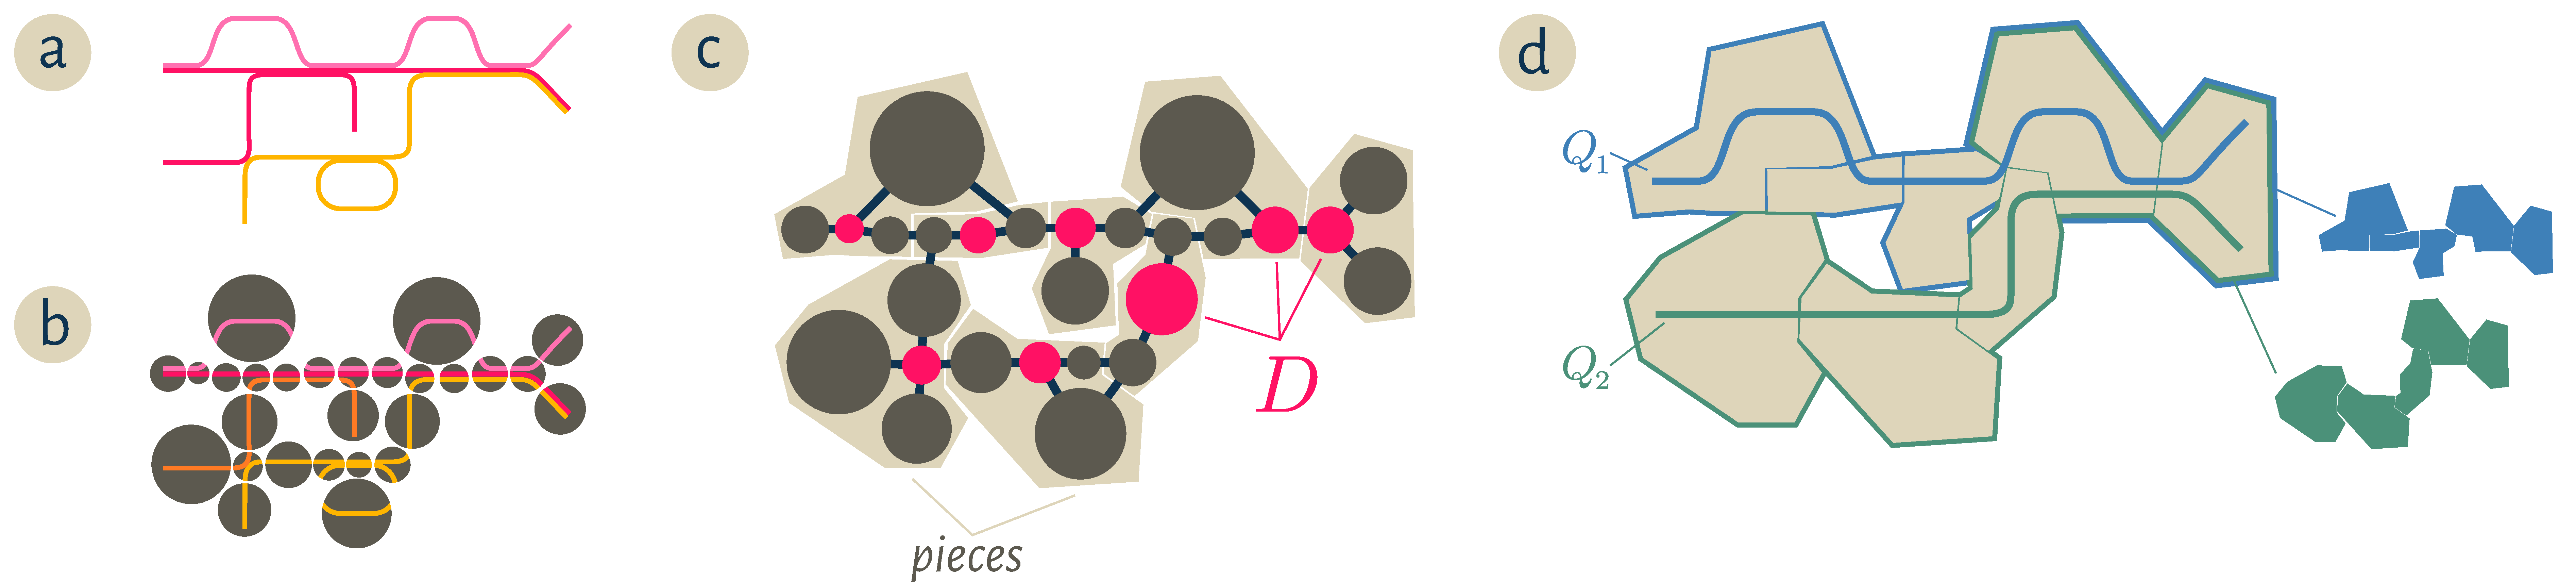
\includegraphics[width=\linewidth]{figures/domset}
	\caption{
 %(Reads ->) genomes -> DBG -> cDBG -> dominating set
 Starting from a collection of genomic sequences (\textbf a), we form an assembly graph
 where nodes represent distinct linear subsequences (\textbf b). In this assembly graph,
 known as a \emph{compact De Bruijn graph}~\cite{lin2016accurate}, nodes may
 represent many k-mers. The original genomic sequences correspond to walks in
 the graph, and shared nodes between the walks represent shared subsequences.
 %walk = path that can cross back on itself; maybe define in footnote?
 %didn't describe what happens at divergence points.
 We then (\textbf c) identify a subset of nodes $D$ called a \emph{dominating set} so that
 every node in the assembly graph is at distance at most one from some member of
 $D$ (marked pink). We further partition the graph into \emph{\pieces}
 by assigning every node to exactly one of the closest members of $D$ (beige regions
 in (\textbf c) and (\textbf d)).
 For a genomic query $Q$, the \emph{neighborhood} of $Q$ in this graph is the
 union of all \pieces which share at least one k-mer with the query. The colorful
 subsets of the pieces in (\textbf d) correspond to the neighborhoods of the
 queries $Q_1, Q_2$.
 }
 \label{fig:domset}
\end{figure*}

\subsection*{Dominating sets enable efficient neighborhood queries in large assembly graphs}

We designed and implemented~\cite{spacegraphcats} a set of algorithms for efficiently
finding content in a metagenome that is close to a query as measured
by distance in a compact De Bruijn graph (cDBG) representation of the
sequencing data (\autoref{fig:domset}). To accomplish this, we organize the cDBG into {\em \pieces}
around a set of \emph{dominators} that are collectively close to all vertices. In this
context, the {\em neighborhood} of a query is the union of all \pieces it overlaps;
to enable efficient search, we build an invertible index of the \pieces.

We compute dominators so that the minimum distance from every vertex
in the cDBG to some dominator is at most $r$ (an \emph{$r$-dominating set})
using~\algoref{alg:r-domset}, which is based on the linear-time approximation algorithm
given by \Dvorak and Reidl~\cite{felixThesis}. Although finding a minimum $r$-dominating set is
NP-hard~\cite{karp1972reducibility,chlebik2008approximation,downey2012parameterized} and
an approximation factor below~$\log n$ is probably impossible~\cite{chlebik2008approximation}
in general graphs, our approach guarantees constant-factor approximations
in linear running time by exploiting the fact that
(compact) De Bruijn graphs have \emph{bounded expansion}, a special type of
sparsity~\cite{sparsity}. \algoref{alg:r-domset} first
annotates the graph to determine the distances between all pairs of vertices at
distance at most $r$ (lines~\ref{algstep:dtf_start}-\ref{algstep:dtf_end}) and
then uses these distances to ensure each vertex is close to a dominator.
The core of the efficient distance computation is based on
\emph{distance-truncated transitive fraternal (dtf) augmentations}~\cite{felixThesis}
which produce a directed graph in which each arc $uv$ is labeled with
$\omega(uv)$, the distance from $u$ to $v$ in the original cDBG.\looseness-1

Importantly, our implementation enhances the algorithm
in~\cite{felixThesis} by computing only $r{-}1$ rounds of dtf-augmentations
instead of~$2r{-}1$. Since augmentation is the computationally most
expensive part of the pipeline and the running time depends non-linearly on
the number of rounds, this vastly improves this algorithm's scalability.
To maintain approximation guarantees on the dominating set size with fewer augmentations,
we introduce a threshold parameter $\texttt{domThreshold}(r)$
which affects the constant factor in our worst-case bound.
We selected a threshold (see Supp. Material) that produces $r$-dominating sets of
comparable size to those computed by the algorithm in~\cite{felixThesis}. Additionally,
we found that processing vertices using a minimum in-degree ordering (line~\ref{algstep:order})
was superior to other common orders (e.g. arbitrary, min/max total degree, max in-degree).\looseness-1

\begin{algorithm}[!b]
	\begin{algorithmic}[1]
		\Require Graph $G$, radius $r$
		\Ensure $r$-dominating set $D$ of $G$
		\State $\vec G_1\leftarrow \texttt{orient}(G)$\label{algstep:dtf_start}
		\For{$i\in 2,\dots, r$}
			\State $\vec G_i\leftarrow \texttt{dtfAugmentation}(\vec G_{i-1})$\label{algstep:dtf_end}
		\EndFor
		\State Initialize $d[v] \leftarrow \infty$ and $c[v] \leftarrow 0$ for all~$v \in G$
		\State $D\leftarrow \emptyset$
		\ForAll{$v\in \vec G_r$ sorted by ascending in-degree}\label{algstep:order}
			\ForAll{$u\in N^{-}(v)$} \label{algstep:pull-loop}
				\State $d[v]\leftarrow\operatorname{min}\left(d[v], d[u]+\omega(uv)\right)$\label{algstep:pull}
			\EndFor
			\If{$d[v]>r$}
				\State $D\leftarrow D\cup \{v\}$ and
					   $d[v]\leftarrow 0$\label{algstep:add_to_domset}\label{algstep:D1}
				\ForAll{$u\in N^-(v)$}\label{algstep:pushloop}
					\State $d[u]\leftarrow \operatorname{min}\left(d[u],\omega(uv)\right)$\label{algstep:push}
					\State $c[u]\leftarrow c[u] + 1$
					\If{$c[u] > \texttt{domThreshold}(r)$}
						\State $D\leftarrow D\cup \{u\}$ and
							   $d[u]\leftarrow 0$\label{algstep:D2}
						\ForAll{$w\in N^-(u)$}
							\State $d[w]\leftarrow \operatorname{min}\left(d[w],\omega(wu)\right)$\label{algstep:D2end}
						\EndFor
					\EndIf
				\EndFor
			\EndIf
		\EndFor
		\State \Return $D$
	\end{algorithmic}
	\caption{$\texttt{rdomset}(G, r)$}\label{alg:r-domset}
\end{algorithm}


After computing an $r$-dominating set $D$ of $G$ with \algoref{alg:r-domset},
\algoref{alg:index_pieces} partitions the vertices of $G$ into pieces so that
each \piece $P[v]$ contains a connected set of vertices for which $v$ is the
closest member of $D$ (\autoref{fig:domset}). Finally, we use minimal perfect
hashing (\texttt{mphfIndex})~\cite{limasset2017mphf} to compute an invertible
index\footnote{an invertible function that defines both an index and the corresponding inverted index}
between \pieces and their sequence content in the metagenome.

One feature of this approach is that the dominating set and index only need to be computed once for a given metagenome, independent of the number and content of anticipated queries.
Queries
can then be performed using \algoref{alg:search} in time that
scales linearly with the size of their {\em neighborhood} --
all genomic content assigned to \pieces that contain part of the query.

Our implementations of these algorithms in \sgc can be run on
metagenomic data with millions of cDBG nodes (\autoref{tab:data});
indexing takes under an hour, enabling queries to complete in seconds
to minutes (\autoref{tab:benchmarking}). See \appendixref{subsec:runtimes}
for full benchmarking (including cDBG construction). This
provides us with a tool to systematically investigate assembly graph
neighborhoods.

% can collapse lines 11-12 and 17-18 similar to line 5 for space saving if necessary
\begin{algorithm}[!h]
	\begin{algorithmic}[1]
		\Require{Metagenome $\mathcal{M}$, radius $r$}
		\Ensure{Invertible index $I \colon \mathcal{M} \to \mathcal{P}$; $\mathcal{P}$ is a set of \pieces}
		\State $G\leftarrow \texttt{cDBG}(\mathcal{M})$\;
		\State $D\leftarrow \texttt{rdomset}(G, r)$\;
		\State Initialize $\delta[v] \leftarrow v$ for all $v \in D$\;
		\State $U \leftarrow V(G) \setminus D$
		\While{$U \neq \emptyset$}\label{algstep:partition_start}
			\For{$v \in V(G) \setminus U$}
				\For{$u \in N(v) \cap U$}
					\State $\delta[u] \leftarrow \delta[v]$\;
					\State $U \leftarrow U \setminus \{u\}$\;
				\EndFor
			\EndFor
		\EndWhile
 		\State $\mathcal{P}[v] \leftarrow \{u:\delta[u] = v\}$\;\label{algstep:partition_end}
		\State $I_{\mathcal{M}} \leftarrow \texttt{mphfIndex}(\mathcal{M}, \mathcal{P})$\;
		\State \Return $I_{\mathcal{M}}$
	\end{algorithmic}
	\caption{$\texttt{indexPieces}(\mathcal{M},r)$}\label{alg:index_pieces}
\end{algorithm}

\begin{algorithm}[!h]
	\begin{algorithmic}[1]
		\Require Index $I_{\mathcal{M}}$, Query $Q$
		\Ensure The query neighborhood $\mathcal{N}_Q$
		\State $\mathcal{N}_Q \leftarrow \bigcup_{k \in Q}I_{\mathcal{M}}^{-1}(I_{\mathcal{M}}(k))$\;
		\State \Return $\mathcal{N}_Q$
	\end{algorithmic}
	\caption{$\texttt{search}(I_{\mathcal{M}}, Q)$}\label{alg:search}
\end{algorithm}


%Figure 2
\begin{figure*}
  \centering
  \subfloat{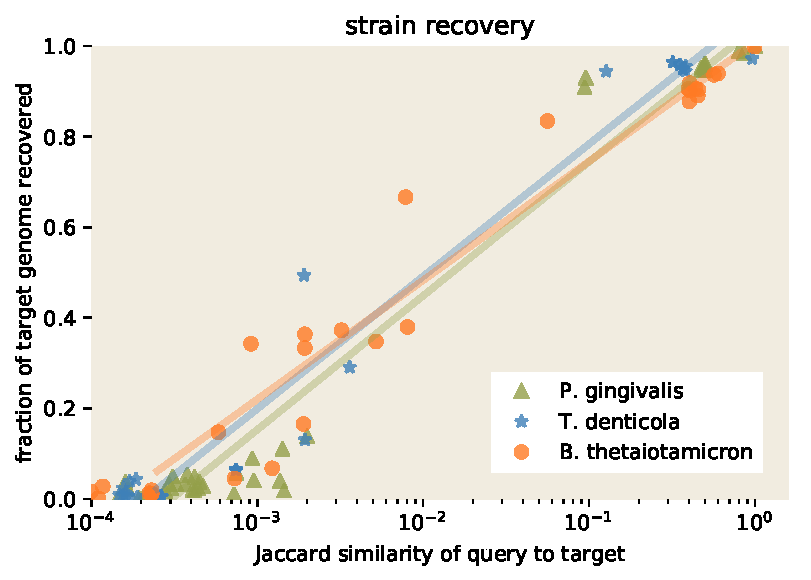
\includegraphics[width=0.4\linewidth,valign=c]{figures/partial_query_a}}%
  \hspace*{2cm}%
  \subfloat{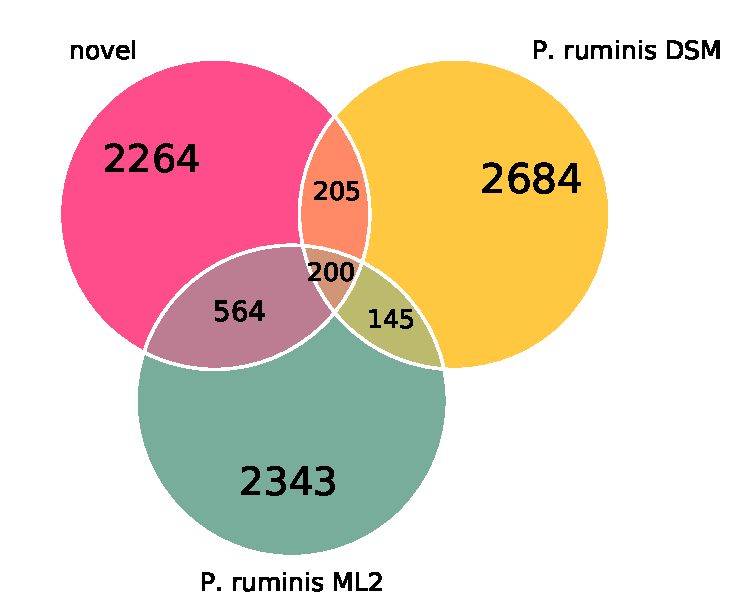
\includegraphics[width=0.3\linewidth,valign=c]{figures/partial_query_b}}%
  \hspace*{1cm}%
	\caption{Neighborhood queries enable recovery of relevant genomic content.
  (a) Left Panel: Recovery of each of three target genomes from \podarv
  using queries at a variety of Jaccard distances from the target. Recovery is
  calculated as containment of target genome in query neighborhood.
  (b) Right Panel: Recovery of novel {\em Proteiniclasticum } content
  from \podarv. Nucleotide content from two of the three known {\em P. ruminis} genomes
  overlapped approximately a megabase of sequence in the query neighborhood,
  which also contained approximately 2.3 Mbp of unknown sequence; the third known genome, {\em P. ruminis CGMCC}, was omitted from the figure as it is 99.7\% similar to {\em P. ruminis DSM}. Numbers are in thousands of k-mers.}\label{fig:partial_query}
\end{figure*}

%Data Set Properties

\begin{table}[t]
	\centering
	\begin{tabular}{l r r r r r}
	\toprule
	Dataset & $|V|$ & $|E|$/$|V|$ & $|D|$ & $\overline{|Q|}$ & $\overline{|\mathcal{P} \cap \mathcal{N}_Q|}$ \\
	\midrule
	\podarv &      916\,041 & 2.2 &    542\,350 & 1\,475\,892 &   4\,106 \\
	\hu     &  13\,852\,950 & 2.6 & 6\,724\,505 & 1\,112\,516 & 106\,091 \\
	\bottomrule
	\end{tabular}
	\caption{Number of cDBG nodes $|V|$, edge density of cDBG $|E|/|V|$, size of $1$-dominating set $|D|$,
	average query size (k-mers) $\overline{|Q|}$, and average number of pieces in query neighborhood $\overline{|\mathcal{P} \cap \mathcal{N}_Q|}$. Queries are the 51 genomes and 23 genome bins fully present in \podarv and \hu, respectively.} \label{tab:data}

	\centering
	\begin{tabular}{l l r r}
	\toprule
	Dataset & Algorithm & Time (s) & Memory (MB) \\
	\midrule
	\multirow{3}{*}{\podarv}
   & \texttt{rdomset}     &  78.1 &  4\,304 \\
   & \texttt{indexPieces} & 359.9 & 14\,108 \\
   & \texttt{search}      &  14.9 &  3\,463 \\
	\multirow{3}{*}{\hu}
   & \texttt{rdomset}     & 1\,181.1 & 60\,238  \\
   & \texttt{indexPieces} &    859.3 & 40\,713  \\
   & \texttt{search}      &     67.9 & 15\,228  \\
	\bottomrule
	\end{tabular}
	\caption{Time and memory usage of \sgc for Algorithms~\ref{alg:r-domset}-\ref{alg:search} on representative metagenome data. The times for \algoref{alg:search} are averaged over all queries (see \autoref{tab:data}).  Statistics reported for \algoref{alg:index_pieces} exclude lines 1-2 of pseudocode. Times are rounded to the nearest tenth of a second; memory is rounded to the nearest Megabyte.}\label{tab:benchmarking}
\end{table}


\subsection*{Neighborhood queries enable recovery of relevant unknown genomic content}
%Use queries that aren't 100% present in the graph to try to retrieve things that are there.

We first measured how well an inexact query can recover a target genome
from a metagenome. For a benchmark data set, we used the
\podarv data set \cite{podar}. This is a ``mock'' metagenome containing
genomes from 65 strains and species of bacteria and archaea, each
grown independently and rendered into DNA, then combined and sequenced
as a metagenome.  This metagenome is a commonly used
benchmark for assembly \cite{Awad155358,megahit,Seah2015,nurk2017metaspades}.

%by querying for a known target genome using queries closely related to the target.
To evaluate the effectiveness of neighborhood query at recovering
strain variants,
we chose three target genomes from \podarv -- {\em Porphyromonas
  gingivalis ATCC 33277}, {\em Treponema denticola ATCC 35405}, and
{\em Bacteroides thetaiotaomicron VPI-5482} -- that have many
taxonomically close relatives in GenBank. We then used these relatives
to query the \podarv mixture and measure the recovery of the target
genome.  The results, in \autoref{fig:partial_query}(a), show that
graph neighborhood query can recover 35\% or more of some target genomes
starting from a relative with Jaccard similarity as low as 1\%: even a
small number of shared k-mers sufficed to define a much larger neighborhood
that contains related genomes.


We next applied neighborhood query to retrieve an unknown genome from \podarv.
Several papers have noted the
presence of unexpected sequence in the assemblies of this data, and
Awad et al. identify at least two species that differ from
the intended mock metagenome contents \cite{megahit,Awad155358}.  One species
variant has partial matches to several different {\em
  Fusobacterium nucleatum} genomes, while the other incompletely matches to
three strains of
{\em Proteiniclasticum ruminis}.

The complete genomes of these two variants are not in public databases and, for
the {\em Proteiniclasticum} variant, cannot
be entirely recovered with existing approaches: when we
assemble the reads that share k-mers with the available genomes, a
marker-based analysis with CheckM estimates that 98.8\% of the {\em
  Fusobacterium} variant is recovered, while only 72.96\% of the {\em
  Proteiniclasticum} variant is recovered. We therefore tried using
neighborhood queries to expand our knowledge of the {\em Proteiniclasticum} variant.

We performed a neighborhood query into \podarv with all three known {\em
  Proteiniclasticum} genomes from GenBank.  We then extracted the reads
overlapping this neighborhood and assembled them with MEGAHIT.  The
retrieved genome neighborhood for {\em Proteiniclasticum} contains
2264K novel k-mers (\autoref{fig:partial_query}(b)). The reads from
the query neighborhood assembled into a 3.1 Mbp genome bin. The
assembly is estimated by CheckM to be 100\% complete, with 10.3\%
contamination.
The mean amino acid identity between {\em P. ruminis ML2} and the
neighborhood assembly is above 95\%, suggesting that this is indeed
the genome of the {\em Proteiniclasticum} variant, and that
neighborhood query retrieves a full draft genome sequence (see Supp. Material~\ref{subsec:aai}).

% FIGURE 3
\begin{figure*}[th]
	\centering
    \subfloat{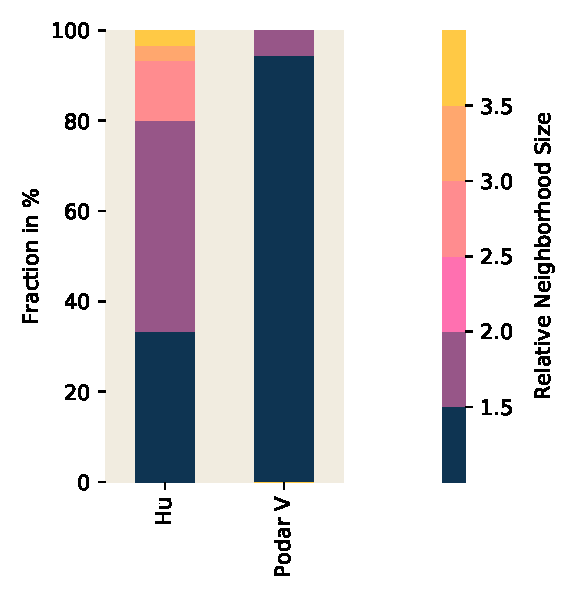
\includegraphics[width=0.34\linewidth]{figures/hu_strain_a}}
    \hspace{.05\linewidth}
    \subfloat{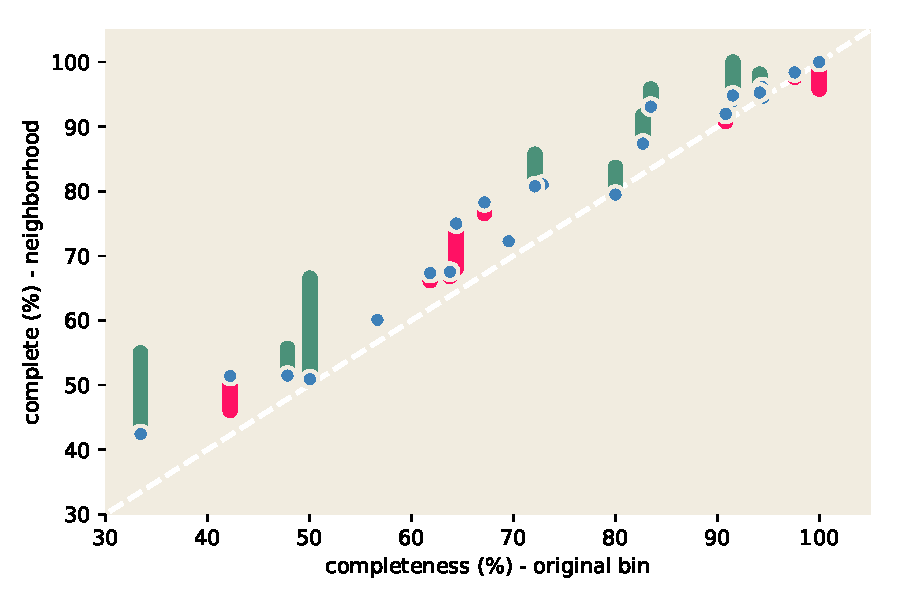
\includegraphics[width=0.55\linewidth]{figures/hu_strain_b}}
	\caption{Query neighborhoods in \hu metagenome are large and contain additional marker genes.
  (a) Left Panel: Neighborhood sizes are larger in \hu than in \podarv. Here
  we queried \podarv and \hu using each of 51 and 23 genomes fully present
  in the respective datasets and measured the relative size of its neighborhood—a
  size of 1 indicates that no additional sequence is present in the neighborhood,
  while a size of 2 indicates that the retrieved neighborhood is twice the size
  of the query genome.
  (b) Right Panel: Query neighborhoods are estimated to be more complete
  than the original genome bins. We queried \hu using each of 23 genomes binned
  from SB1, and assembled the resulting neighborhoods using MEGAHIT and \plass.
  The blue points represent completeness estimates of MEGAHIT-assembled
  neighborhoods, while green and pink bars represent the additional or missing
  content in the \plass assemblies respectively.
  }\label{fig:hu_strain}
\end{figure*}



\subsection*{Query neighborhoods in a real metagenome do not always assemble well}

Real metagenomes may differ substantially from mock metagenomes in
size, complexity, and content.  In particular, real metagenomes may
contain a complex mixture of species and strain variants \cite{Sharon2015}
and the performance of assembly and binning algorithms on these data sets
is challenging to evaluate in the absence of ground truth.
One recent comparison of single-cell genomes and metagenome-assembled
genomes in an ocean environment found that up to 40\% of single-cell
genome content may be missing in metagenome-assembled genomes \cite{baltic}.

We first ask whether genome query neighborhood sizes in a real
metagenome differ from mock metagenomes.  We examined genomes inferred
from the SB1 sample from the Hu et al.\ (2016) study, in which 6
metagenomic samples taken from various types of oil reservoirs were
sequenced, assembled, binned, and computationally analyzed for
biochemical function \cite{Hu2016}.  Examining the 23 binned genomes
in GenBank originating from the SB1 sample, we compared the \hu
neighborhood size distribution with the \podarv data set
(\autoref{fig:hu_strain}(a)). We saw that more genome bins in \hu
have 1.5x or larger query neighborhoods than do the genomes in
\podarv. This suggests the presence of considerably more local
neighborhood content in the real metagenome than in the mock
metagenome.

We next investigated metagenomic content in the query
neighborhoods.  As with the unknown variants in \podarv, we used
CheckM to estimate genome bin completeness.  The estimated bin
completeness for many of the query genomes is low
(\appendixref{subsec:checkm}).
To see if the query neighborhoods contain missing marker genes, we
assembled reads from the query neighborhoods using MEGAHIT.  However,
we found little improvement in the completion metrics (\autoref{fig:hu_strain}(b)).

Investigating further, we found that the query neighborhood assemblies
contain only between 4\% and 56\% of the neighborhood k-mer
content (\appendixref{subsec:inclusion}), suggesting that MEGAHIT is
not including many of the reads in the assembly of the query neighborhoods.
This could result from high
error rates and/or high strain variation in the underlying reads
\cite{CAMI,Awad155358}.

To attempt the recovery of more gene content from the assemblies, we turned to
the \plass amino acid assembler \cite{plass}. \plass implements an
overlap-based amino acid assembly approach that is considerably more
sensitive than nucleotide assemblers and could be more robust to
errors and strain variation \cite{spa}.

When we applied \plass to the reads from the query neighborhoods, we saw
a further increase in neighborhood completeness
(\autoref{fig:hu_strain}(b)).  This suggests that the genome bin
query neighborhoods contain real genes that are accessible to the
\plass amino acid assembler.  We note that these are unlikely to be
false positives, since CheckM uses a highly specific Hidden Markov Model
(HMM)-based
approach to detecting marker genes \cite{CheckM}.

%FIGURE 4
\begin{figure*}[!h]
	% \centering
    \subfloat{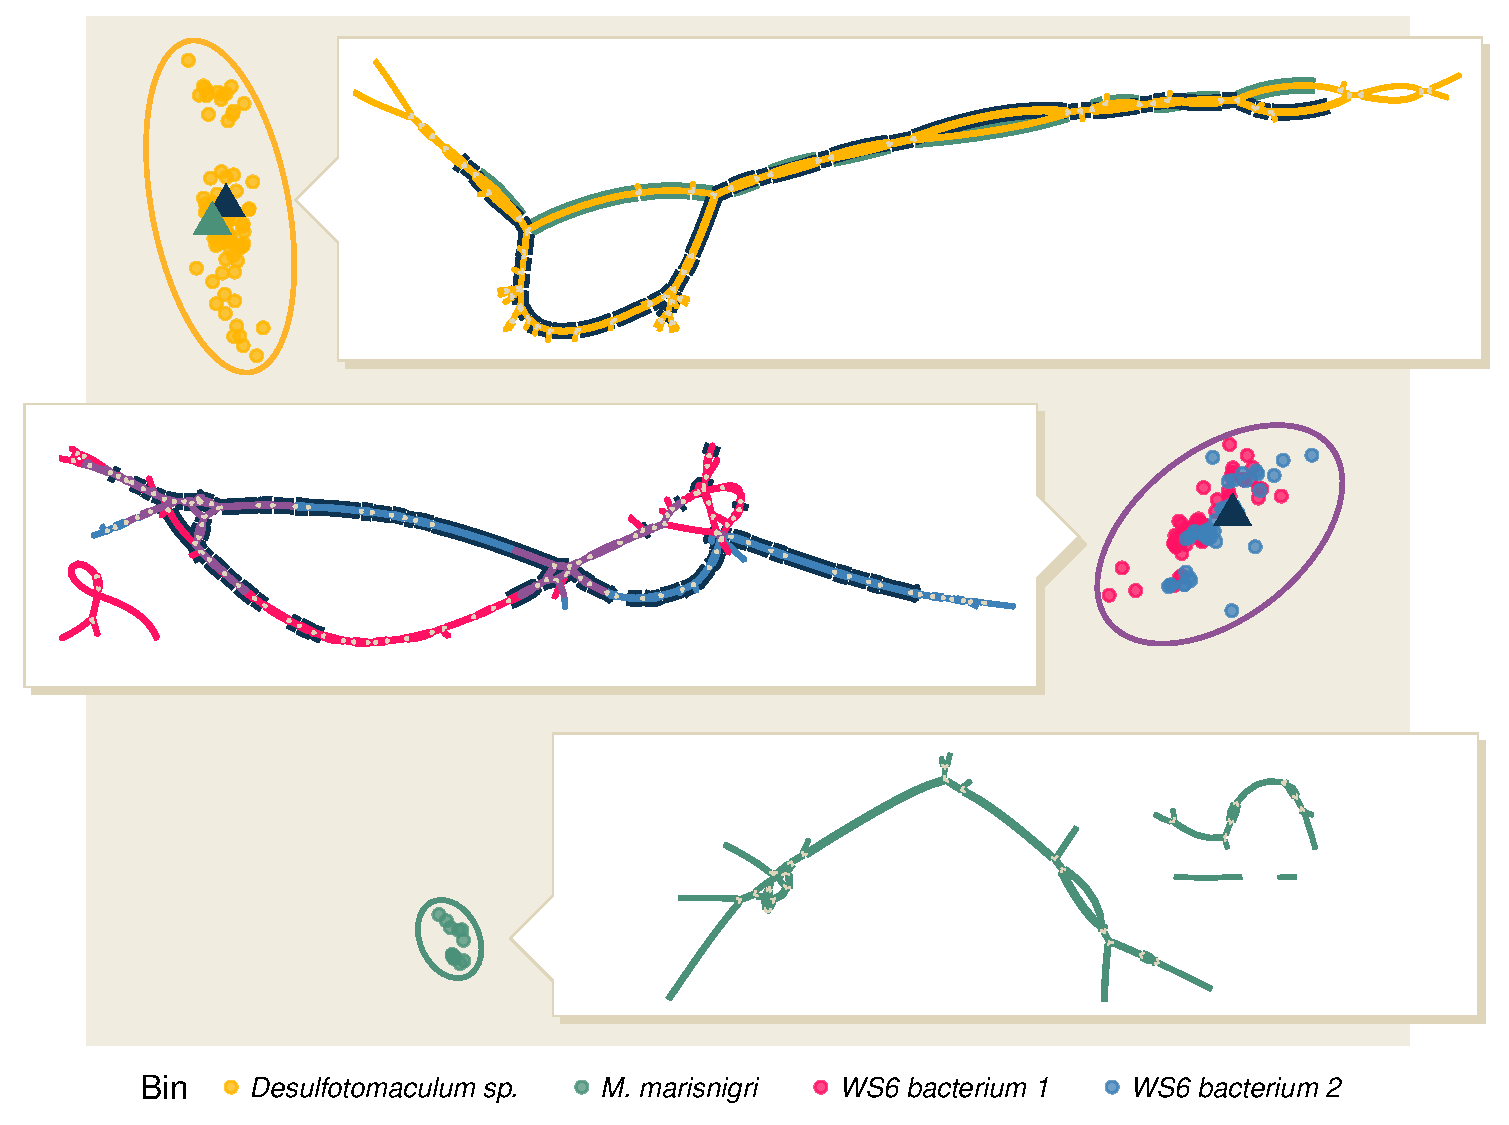
\includegraphics[width=0.54\linewidth]{figures/hu_content_a}}\hspace*{0.01\linewidth}%
    \subfloat{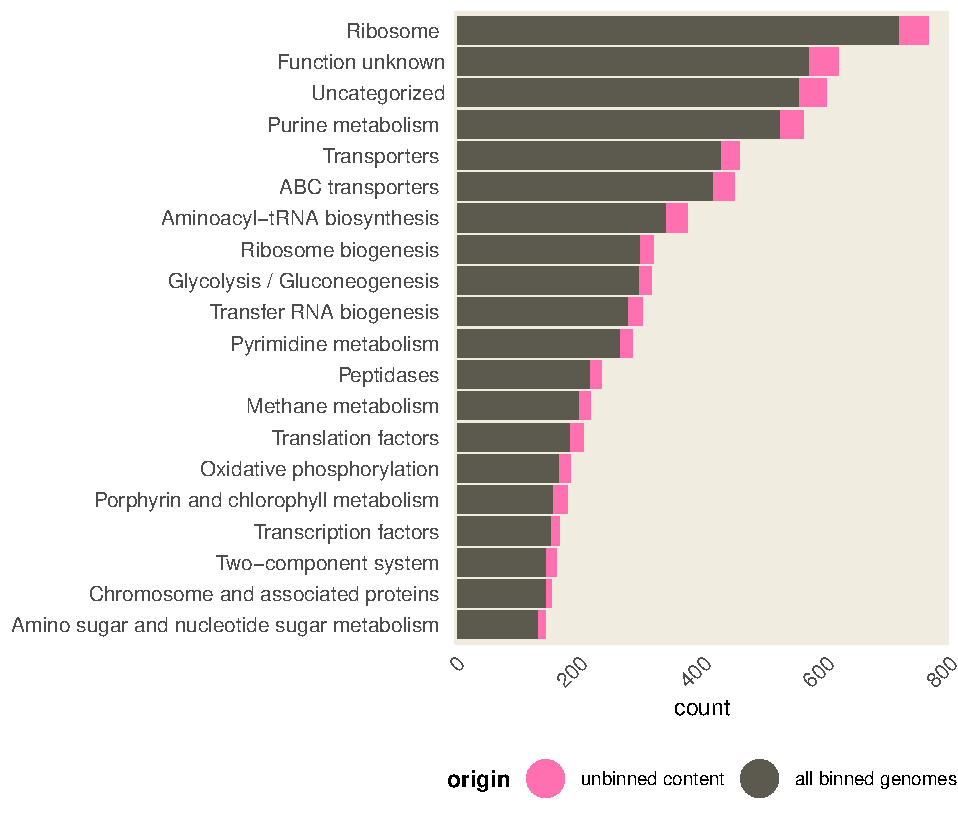
\includegraphics[width=0.45\linewidth]{figures/hu_content_b}}
    \caption{Query neighborhoods in \hu contain sequence variants and new genes.
      (a) Left Panel: gyrA has substantial minor sequence variation in several
      query neighborhoods. In this multidimensional scaling plot, each point
      represents a distinct gyrA sequence from the \plass assemblies of four
      representative query neighborhoods, colored by query binned genome.
      The triangles represent gyrA sequences originating from the
      query binned genome, if any are present.  The inlays
      are visualizations of assembly graphs of reads that contain {\em gyrA}
      sequence in each neighborhood. Unitigs are colored by their cluster of origin;
      matches to {\em gyrA} sequences from the bin are highlighted using color from relevant triangle.
      (b) Right Panel: Genome neighborhoods re-associate annotated
    functionality to binned genomes. For each of 23 genome bins
    originating from \hu, we found the unbinned content by removing all
    orthologs found in the binned genomes in \cite{hu} and by counting distinct
    ortholog annotations once. Functional content is
    distributed throughout pathways present in the binned genomes,
    and increases functionality associated with binned genomes by
    approximately 13\%.}
  \label{fig:hu_content}
\end{figure*}


\subsection*{Some query neighborhoods contain substantial strain variation}

If strain variation is contributing to poor nucleotide assembly of
marker genes in the query neigborhoods, then \plass should
assemble these variants into similar amino acid sequences.
Strain variation for unknown genes can be difficult to study due to
lack of ground truth, but highly conserved proteins should be readily
identifiable.

The {\em gyrA} gene encodes an essential DNA topoisomerase that
participates in DNA supercoiling and was used by \cite{Hu2016} as a
phylogenetic marker.  In the GenBank bins, we found that 15 of the 23
bins contain at least one gyrA sequence (with 18 {\em gyrA} genes
total).  We therefore used {\em gyrA} for an initial analysis of the
\plass-assembled neighborhood content for all 23 bins.  To avoid confounding effects of
random sequencing error in the analysis and increase specificity at the
cost of sensitivity, we focused only on high-abundance data:
we truncated all reads
in the query neighborhoods at any k-mer that appears fewer than five
times, and ran \plass on these abundance-trimmed reads from each
neighborhood.  We then searched the gene assemblies with a gyrA-derived
HMM, aligned all high-scoring matches, and calculated a pairwise similarity
matrix from the resulting alignment.\looseness-1
%TER add in k-mer size of 31 into materials and methods

When we examine all of the high-scoring gyrA protein matches in the
hard-trimmed data, we see
considerable sequence variation in some query neighborhoods
(\autoref{fig:hu_content}(a)). Much of this variation is present in
fragmented \plass assemblies; when the underlying nucleotide sequences
are retrieved and used to construct a compact De Bruijn graph, the
variation is visible as spurs off of a few longer paths (insets in
\autoref{fig:hu_content}(a)). When we count the number of
well-supported amino acid variants in isolated positions (i.e. ignoring linkage between variants)
we see that ten of the 23 neighborhoods have an increased number of gyrA
genes, with four neighborhoods gaining a gyrA where none exists in
the bin (\appendixref{subsec:gyrAnbhd}; see lowest inset
in \autoref{fig:hu_content}(a) for one example). Only one
neighborhood, {\em M. bacterium}, loses its gyrA genes due to the
stringent k-mer abundance trimming.
Collectively, the use of the \plass assembler on genome
neighborhoods substantially increases the number of gyrA sequences associated with bins.
% To calculate max # distinct gyrA, see code in misc/distinct_positions.ipynb.

We see this same pattern for many genes, including {\em alaS}, {\em gyrB},
{\em rpb2}
domain 6, {\em recA}, {\em rplB}, and {\em rpsC} (\appendixref{subsec:othergenes}).
This shows that multiple variants of those proteins are present within
at least some of the neighborhoods and implies the presence of
underlying nucleotide strain variation.
This strain variation may be
one reason that nucleotide assembly performs poorly: on average, only
19.6\% of \plass-assembled proteins are found within the nucleotide
assemblies.
% to calculate this number, see misc/plass-in-nucleotide-assemblies.md.

\subsection*{Query neighborhoods assembled with \plass contain additional functional content}

In addition to capturing variants close to sequences in the bins, we
identify many novel genes in the query neighborhoods. We used KEGG to
annotate the \plass-assembled amino acid sequences, and subtracted any
homolog already annotated in the genome bin.
We also ignoreed homolog abundance such that each homolog is counted only
once per neighborhood.

Novel functional content is distributed throughout pathways present in
the genome bins, and increases functionality associated with binned
genomes by approximately 13\% (\autoref{fig:hu_content}(b)).  This
includes orthologs in biologically relevant pathways
such as methane metabolism, which are important for biogeochemical
cycling in oil reservoirs \cite{Hu2016}.

Genes in these neighborhoods contain important metabolic functionality expanding
the pathways already identified in \cite{Hu2016}. We find 40
unique orthologs involved in nitrogen fixation across eight
neighborhoods, four of which had no ortholog in the bin.  Importantly,
we find the ratio of observed orthologs approximately matches that
noted in \cite{Hu2016}, where two thirds of nitrogen fixation
functionality is attributable to archaea (29 of 40 orthologs). This is
in contrast to most ecological systems where bacteria are the dominant
nitrogen fixers \cite{Hu2016}.
